\documentclass[14pt]{extbook}
\usepackage{multicol, enumerate, enumitem, hyperref, color, soul, setspace, parskip, fancyhdr} %General Packages
\usepackage{amssymb, amsthm, amsmath, latexsym, units, mathtools} %Math Packages
\everymath{\displaystyle} %All math in Display Style
% Packages with additional options
\usepackage[headsep=0.5cm,headheight=12pt, left=1 in,right= 1 in,top= 1 in,bottom= 1 in]{geometry}
\usepackage[usenames,dvipsnames]{xcolor}
\usepackage{dashrule}  % Package to use the command below to create lines between items
\newcommand{\litem}[1]{\item#1\hspace*{-1cm}\rule{\textwidth}{0.4pt}}
\pagestyle{fancy}
\lhead{Makeup Progress Quiz 2}
\chead{}
\rhead{Version C}
\lfoot{5763-3522}
\cfoot{}
\rfoot{Spring 2021}
\begin{document}

\begin{enumerate}
\litem{
Graph the equation below.\[ f(x) = (x+1)^2 - 18 \]\begin{enumerate}[label=\Alph*.]
\begin{multicols}{2}\item 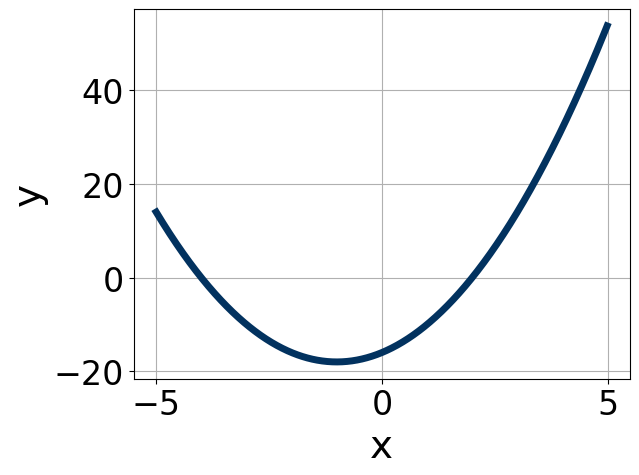
\includegraphics[width = 0.3\textwidth]{../Figures/quadraticEquationToGraphAC.png}\item 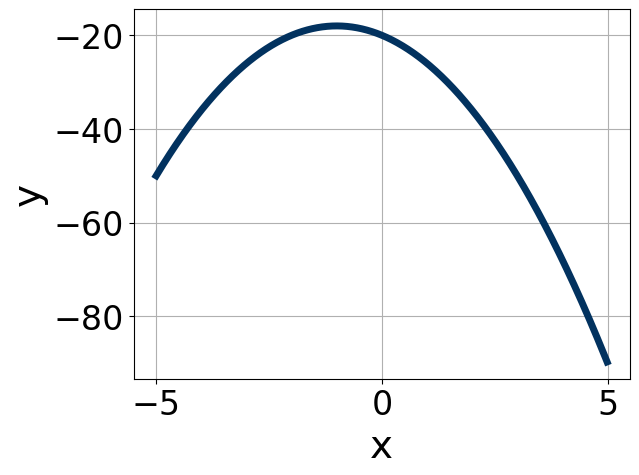
\includegraphics[width = 0.3\textwidth]{../Figures/quadraticEquationToGraphBC.png}\item 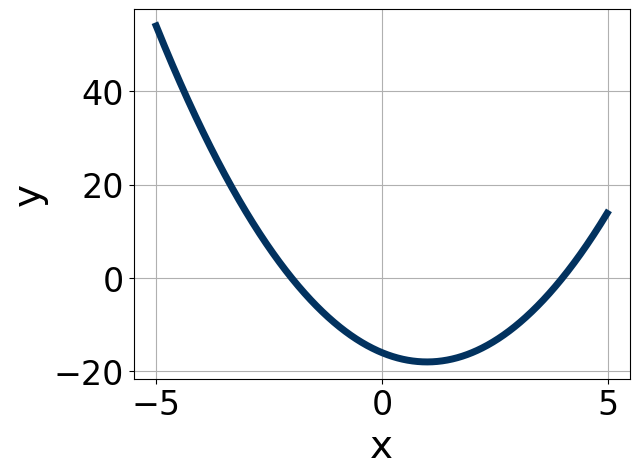
\includegraphics[width = 0.3\textwidth]{../Figures/quadraticEquationToGraphCC.png}\item 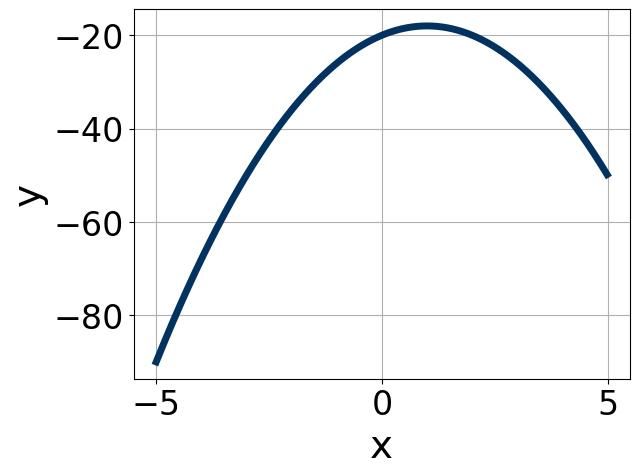
\includegraphics[width = 0.3\textwidth]{../Figures/quadraticEquationToGraphDC.png}\end{multicols}\item None of the above.
\end{enumerate} }
\litem{
Write the equation of the graph presented below in the form $f(x)=ax^2+bx+c$, assuming  $a=1$ or $a=-1$. Then, choose the intervals that $a, b,$ and $c$ belong to.
\begin{center}
    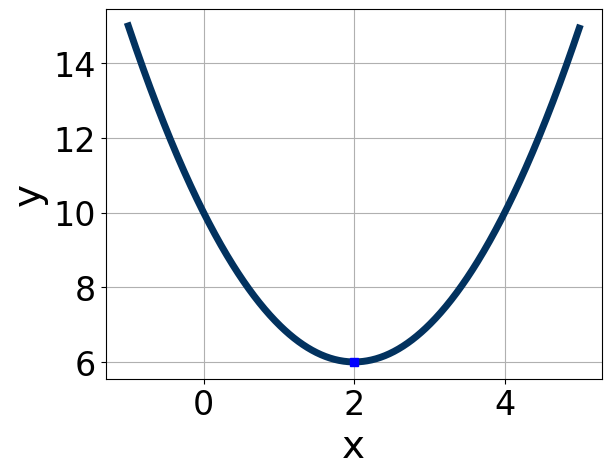
\includegraphics[width=0.5\textwidth]{../Figures/quadraticGraphToEquationC.png}
\end{center}
\begin{enumerate}[label=\Alph*.]
\item \( a \in [1, 3], \hspace*{5mm} b \in [4, 5], \text{ and } \hspace*{5mm} c \in [7, 15] \)
\item \( a \in [1, 3], \hspace*{5mm} b \in [4, 5], \text{ and } \hspace*{5mm} c \in [-3, -1] \)
\item \( a \in [-1, 0], \hspace*{5mm} b \in [-8, -1], \text{ and } \hspace*{5mm} c \in [1, 4] \)
\item \( a \in [-1, 0], \hspace*{5mm} b \in [4, 5], \text{ and } \hspace*{5mm} c \in [1, 4] \)
\item \( a \in [1, 3], \hspace*{5mm} b \in [-8, -1], \text{ and } \hspace*{5mm} c \in [7, 15] \)

\end{enumerate} }
\litem{
Solve the quadratic equation below. Then, choose the intervals that the solutions $x_1$ and $x_2$ belong to, with $x_1 \leq x_2$.\[ 25x^{2} +50 x + 24 = 0 \]\begin{enumerate}[label=\Alph*.]
\item \( x_1 \in [-30.53, -29.87] \text{ and } x_2 \in [-20, -19.97] \)
\item \( x_1 \in [-1.66, -1.29] \text{ and } x_2 \in [-0.7, -0.51] \)
\item \( x_1 \in [-1.33, -1.13] \text{ and } x_2 \in [-0.88, -0.74] \)
\item \( x_1 \in [-2.57, -1.79] \text{ and } x_2 \in [-0.46, -0.23] \)
\item \( x_1 \in [-6.85, -5.53] \text{ and } x_2 \in [-0.23, -0.13] \)

\end{enumerate} }
\litem{
Solve the quadratic equation below. Then, choose the intervals that the solutions belong to, with $x_1 \leq x_2$ (if they exist).\[ -14x^{2} +14 x + 2 = 0 \]\begin{enumerate}[label=\Alph*.]
\item \( x_1 \in [-1.75, -0.34] \text{ and } x_2 \in [0.04, 0.29] \)
\item \( x_1 \in [-0.57, 0.68] \text{ and } x_2 \in [1.05, 1.43] \)
\item \( x_1 \in [-15.94, -15.57] \text{ and } x_2 \in [1.72, 2.15] \)
\item \( x_1 \in [-17.29, -15.97] \text{ and } x_2 \in [17.86, 18.31] \)
\item \( \text{There are no Real solutions.} \)

\end{enumerate} }
\litem{
Graph the equation below.\[ f(x) = (x+4)^2 - 14 \]\begin{enumerate}[label=\Alph*.]
\begin{multicols}{2}\item 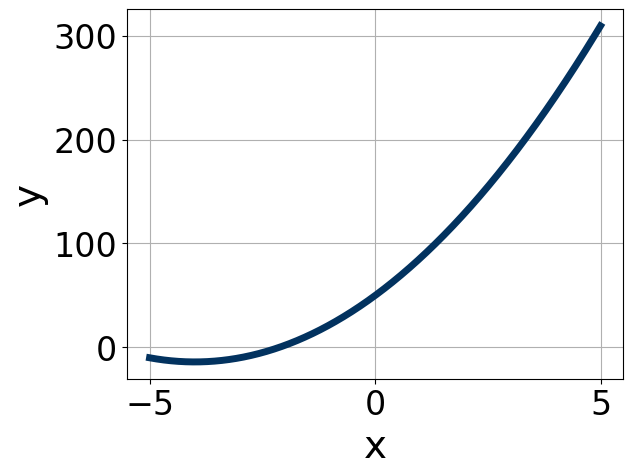
\includegraphics[width = 0.3\textwidth]{../Figures/quadraticEquationToGraphCopyAC.png}\item 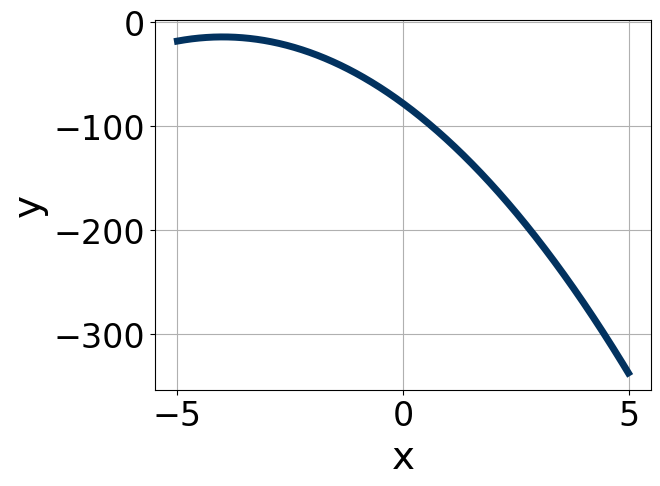
\includegraphics[width = 0.3\textwidth]{../Figures/quadraticEquationToGraphCopyBC.png}\item 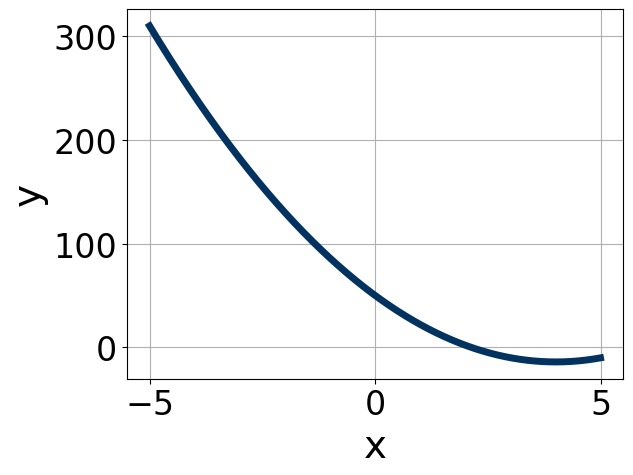
\includegraphics[width = 0.3\textwidth]{../Figures/quadraticEquationToGraphCopyCC.png}\item 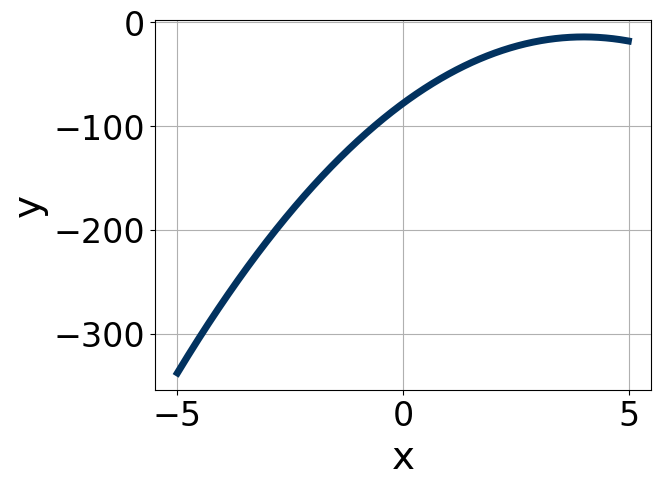
\includegraphics[width = 0.3\textwidth]{../Figures/quadraticEquationToGraphCopyDC.png}\end{multicols}\item None of the above.
\end{enumerate} }
\litem{
Factor the quadratic below. Then, choose the intervals that contain the constants in the form $(ax+b)(cx+d); b \leq d.$\[ 81x^{2} -54 x + 8 \]\begin{enumerate}[label=\Alph*.]
\item \( a \in [8.4, 9.6], \hspace*{5mm} b \in [-5, -3], \hspace*{5mm} c \in [8, 14], \text{ and } \hspace*{5mm} d \in [-4, 1] \)
\item \( a \in [26.7, 28.6], \hspace*{5mm} b \in [-5, -3], \hspace*{5mm} c \in [2, 5], \text{ and } \hspace*{5mm} d \in [-4, 1] \)
\item \( a \in [-1.7, 1.6], \hspace*{5mm} b \in [-40, -31], \hspace*{5mm} c \in [0, 2], \text{ and } \hspace*{5mm} d \in [-24, -16] \)
\item \( a \in [2.8, 4.7], \hspace*{5mm} b \in [-5, -3], \hspace*{5mm} c \in [20, 30], \text{ and } \hspace*{5mm} d \in [-4, 1] \)
\item \( \text{None of the above.} \)

\end{enumerate} }
\litem{
Write the equation of the graph presented below in the form $f(x)=ax^2+bx+c$, assuming  $a=1$ or $a=-1$. Then, choose the intervals that $a, b,$ and $c$ belong to.
\begin{center}
    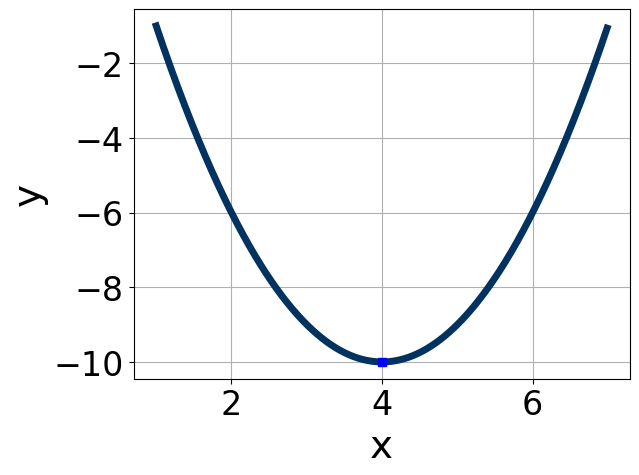
\includegraphics[width=0.5\textwidth]{../Figures/quadraticGraphToEquationCopyC.png}
\end{center}
\begin{enumerate}[label=\Alph*.]
\item \( a \in [-2.6, 0.2], \hspace*{5mm} b \in [8, 9], \text{ and } \hspace*{5mm} c \in [-28, -23] \)
\item \( a \in [0.5, 3.6], \hspace*{5mm} b \in [8, 9], \text{ and } \hspace*{5mm} c \in [4, 7] \)
\item \( a \in [-2.6, 0.2], \hspace*{5mm} b \in [-9, -5], \text{ and } \hspace*{5mm} c \in [-28, -23] \)
\item \( a \in [0.5, 3.6], \hspace*{5mm} b \in [-9, -5], \text{ and } \hspace*{5mm} c \in [4, 7] \)
\item \( a \in [0.5, 3.6], \hspace*{5mm} b \in [8, 9], \text{ and } \hspace*{5mm} c \in [24, 28] \)

\end{enumerate} }
\litem{
Factor the quadratic below. Then, choose the intervals that contain the constants in the form $(ax+b)(cx+d); b \leq d.$\[ 81x^{2} +18 x -8 \]\begin{enumerate}[label=\Alph*.]
\item \( a \in [24.4, 27.2], \hspace*{5mm} b \in [-6, 1], \hspace*{5mm} c \in [1.7, 3.4], \text{ and } \hspace*{5mm} d \in [4, 5] \)
\item \( a \in [8.5, 9.8], \hspace*{5mm} b \in [-6, 1], \hspace*{5mm} c \in [8.6, 10.4], \text{ and } \hspace*{5mm} d \in [4, 5] \)
\item \( a \in [2.9, 3.9], \hspace*{5mm} b \in [-6, 1], \hspace*{5mm} c \in [25.7, 28.6], \text{ and } \hspace*{5mm} d \in [4, 5] \)
\item \( a \in [0.3, 1.6], \hspace*{5mm} b \in [-24, -15], \hspace*{5mm} c \in [-0.1, 2.8], \text{ and } \hspace*{5mm} d \in [31, 38] \)
\item \( \text{None of the above.} \)

\end{enumerate} }
\litem{
Solve the quadratic equation below. Then, choose the intervals that the solutions belong to, with $x_1 \leq x_2$ (if they exist).\[ 10x^{2} +14 x + 2 = 0 \]\begin{enumerate}[label=\Alph*.]
\item \( x_1 \in [-12.2, -9] \text{ and } x_2 \in [9.7, 11.2] \)
\item \( x_1 \in [-14.1, -12] \text{ and } x_2 \in [-2.3, -1.5] \)
\item \( x_1 \in [-1.6, -0.4] \text{ and } x_2 \in [-0.6, 0.6] \)
\item \( x_1 \in [0, 1.4] \text{ and } x_2 \in [0.5, 1.9] \)
\item \( \text{There are no Real solutions.} \)

\end{enumerate} }
\litem{
Solve the quadratic equation below. Then, choose the intervals that the solutions $x_1$ and $x_2$ belong to, with $x_1 \leq x_2$.\[ 12x^{2} +43 x + 36 = 0 \]\begin{enumerate}[label=\Alph*.]
\item \( x_1 \in [-2.47, -0.85] \text{ and } x_2 \in [-1.41, -1.23] \)
\item \( x_1 \in [-27.71, -26.78] \text{ and } x_2 \in [-16.07, -15.98] \)
\item \( x_1 \in [-3.42, -2.66] \text{ and } x_2 \in [-1.26, -0.96] \)
\item \( x_1 \in [-7.02, -6.44] \text{ and } x_2 \in [-0.62, -0.38] \)
\item \( x_1 \in [-9.86, -7.86] \text{ and } x_2 \in [-0.41, -0.26] \)

\end{enumerate} }
\end{enumerate}

\end{document}